\problemname{Raktuvjtrīce}
\illustration{.4}{img/Goodluck_Mine.jpg}{%
  \emph{Veiksmes raktuve, Eja}, Ashley Dace. 
  License CC BY-SA 2.0.}

\noindent

Pilnīgi autonomās alus mikrodarītavas, kas uzstādītas pamestajās Moravijas rūķu raktuvēs, patiesi ir pierādījums rūķu atjautībai un meistarībai!
Diemžēl dažreiz raktuves tiek satricinātas ar zemestrīcēm, kas izraisa cauruļvadu un piltuvju novirzes, kā rezultātā dārgais dzēriens izlīst uz grīdas.
Kā Cildenam Alus Darītavas Drošības Uzraugam, jūsu pienākums izslēgt ierīces visās zālēs, ja notiek zemestrīce.

Tuneļu caurstaigāšana aizņem laiku, tāpēc jūs neizbēgami ieradīsīties pie daudzām ierīcēm ar nokavēšanos.
No tā nevar izvairīties, bet jūs vēlaties minimizēt kopējo izlijušā dzēriena daudzumu.

\medskip
Rūķu raktuves sastāv no $n$~zālēm, kas savienotas ar $n-1$ tuneļiem.
Visa sistēma ir savienota, tāpēc ir iespējams nokļūt no jebkuras zāles līdz jebkurai citai.
Viena tuneļa caurstaigāšana aizņem $1$ laika vienību.
Ierīču izslēgšana un zāles caurceļošana neprasa laiku.
Ja zālē ierīces tiek atslēgtas laikā $t$ pēc zemestrīces, tas izraisīs $t$~litrus izlijušā dzēriena tajā zālē.
Ir tieši viena zemestrīce, kas skar visas zāles vienlaicīgi, un jūs nevarat izslēgt nevienu ierīci pirms zemestrīces.
Jūs varat sākt jebkurā no zālēm.

\section*{Piemērs}

$1$.~piemērā raktuves izskatīsies šādi:

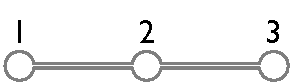
\includegraphics[width=.2\textwidth]{img/sample-1.pdf}

Ja sākt $2$.~zālē un apmeklēt pārējās zāles secībā $2$., $1$., $2$., $3$., tad var izslēgt ierīces tajās laikā $0$ ($2$.~zālē), laikā $1$ ($1$.~zālē) un laikā $3$ ($3$.~zālē).
Tas kopumā izšķiež $0+1+3=4$ litrus dzēriena.
Ja sākt $1$.~zālē un apmeklēt zāles secībā $1$., $2$., $3$., tad kopējais izšķērdētā dzēriena daudzums būs $0+1+2=3$ litri, kas ir labāk.

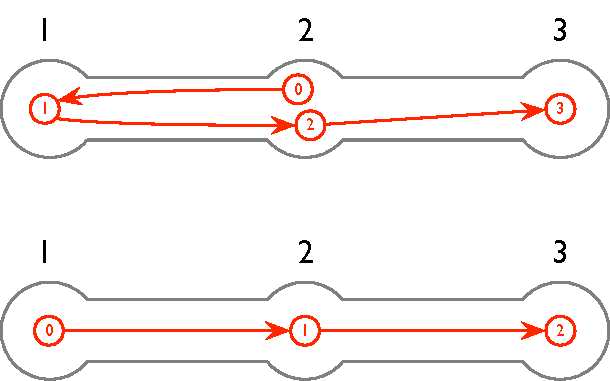
\includegraphics[width=.4\textwidth]{img/sample-1-ans.pdf}

\section*{Ievads}

Ievada pirmā rinda satur veselu skaitli $n$, kas apzīmē zāļu skaitu.
Tiek pieņemts, ka zāles tiek numurētas ar skaitļiem $1$, $\ldots$, $n$.
Nākāmās $n-1$ rindas katra satur divus ar atstarpi atdalītus veselus skaitļus $u$ un $v$ ar 
$1\leq u < v \leq n$, % constraint:hallnames
kas nozīmē, ka zāles~$u$ un~$v$ ir savienotas ar tuneli.

\section*{Izvads}

Izvadiet vienu veselu skaitli, vismazāko iespējamo izlītā dzēriena daudzumu litros.

\section*{Ierobežojumi un vērtēšana}

Vienmēr izpildās ierobežojums
$1\leq n\leq 10^5$. % constraint:n

Jūsu risinājums tiks pārbaudīts uz vairākām testu grupām. Katra grupa ir vērta noteiktu punktu skaitu.
Katra testu grupa satur vairākus testus.
Lai saņemtu punktus par testu grupu, ir jāatrisina visi testi testu grupā.
Jūsu gala rezultāts būs lielākais punktu skaits, kas iegūts ar vienu risinājuma iesniegumu.

\medskip
\begin{tabular}{lll}
Grupa & Punkti & Ierobežojumi \\\hline
  $1$ & $18$ & katra zāle ir savienota ar ne vairāk kā diviem tuneļiem\\
  $2$ & $19$ & ir ne vairāk kā viena zāle, kas savienota ar vairāk kā diviem tuneļiem\\
  $3$ & $20$ & $n\leq 10$\\
  $4$ & $21$ & $n\leq 1000$\\
  $5$ & $22$ & \emph{Bez papildu ierobežojumiem}
\end{tabular}
